\chapter{Analyse, conception, et choix techniques}

Pour conduire ce projet, nous avons opté pour la méthode de gestion de projet Scrum\footnote{Ken Schwaber et Jeff Sutherland, « Scrum Guide ». Scrum.org, 2013 p. 4.} qui est un schéma d’organisation de développement de produits complexes considérée comme une pratique agile; pratique qui implique au maximum le demandeur (client) et permet une grande réactivité à ses demandes. Scrum est défini comme un cadre de travail suivant un cycle de développement itératif, incrémental et adaptatif. S’appuyant sur le découpage d'un projet en boîtes de temps, nommées « sprints » pouvant durer entre quelques heures et un mois (avec une préférence pour deux semaines). Chaque sprint commence par une estimation suivie d'une planification opérationnelle et se termine par une démonstration de ce qui a été achevé.

\section{Analyse des besoins} 

L’analyse consiste à l’aboutissement de l’élaboration d’une solution technique à partir de l’étude des besoins. C’est la première phase du cycle de développement d’un logiciel. Elle sert à identifier les acteurs du système et leur associer chacun l’ensemble des actions avec lesquelles il intervient dans l’objectif de donner un résultat optimal et satisfaisant au client.

\subsection{Les besoins fonctionnels}

Les besoins fonctionnels répondent aux points précis du cahier de charges et sont donc requis par le client. Ils constituent le besoin primaire du client et définissent une fois résolu l’opérationnalité du système. Ainsi l’application doit permettre :

\paragraph{au visiteur de :}
\begin{itemize}
\item[\textbullet] gérer les informations de son compte
\item[\textbullet] consulter l’ensembles des offres d’appartements
\item[\textbullet] consulter l’ensembles des offres d'expériences
\item[\textbullet] réserver un appartement ou une partie d’appartement
\item[\textbullet] s’inscrire à une expérience
\item[\textbullet] prendre connaissances des tarifs
\item[\textbullet] payer une réservation
\item[\textbullet] reporter ou annuler une réservation dans les délai autorisés
\item[\textbullet] consulter l’historique de ses réservations et paiements
\item[\textbullet] demander le titre d’hôte
\item[\textbullet] poster un commentaire
\item[\textbullet] noter un d’hôte ou un logement
\item[\textbullet] recevoir des notifications et rappels
\end{itemize}


\paragraph{à l'hôte de :}
\begin{itemize}
\item[\textbullet] faire tout ce que peut faire un ‘’visiteur’’
\item[\textbullet] mettre en ligne des offres d’appartements ou de parties d’appartement
\item[\textbullet] proposer des expériences thématiques
\item[\textbullet] consulter son historique de réservations
\item[\textbullet] reporter ou annuler une réservation dans les délais autorisés
\item[\textbullet] noter un visiteur
\item[\textbullet] recevoir des paiements
\item[\textbullet] recevoir des notifications
\end{itemize} 

\paragraph{à l’administrateur}
\begin{itemize}
\item[\textbullet] d’accorder le titre d’hôte
\item[\textbullet] de retirer le titre d’hôte
\item[\textbullet] valider un commentaire
\item[\textbullet] d’envoyer les notifications
\item[\textbullet] d’interdire le report ou l’annulation d’une réservation à moins de 24 heures du jour
\end{itemize} 


\subsection{Les besoins non fonctionnels} 
Ces besoins sont soit des besoins optionnels soit des besoins/contraintes liés à l’implémentation. Ainsi, il faudra que l’application soit:
\begin{itemize}
\item[\textbullet] Sécurisée
\item[\textbullet] Dotés d’une bonne expérience utilisateur
\item[\textbullet] Performante
\end{itemize}

La version mobile devra être :
\\Compatible a tout système Android de version minimum 4.3
\\La version web, quand à elle, devra être:
\\Responsive design et compatible à la plupart des navigateurs
\newpage
\section{Choix de la méthode d'analyse} 

Pour la réalisation de notre application, nous avons besoin de gérer des données. De ce fait, l'utilisation d'une base de données est nécessaire. Selon Bouhaddaoui et al. (2010-2011)\footnote{Bouhaddaoui (M. Y.) et Tarek El Allam (M.) « Etude comparative sur les méthodes de modélisation: Comparatif UML - Merise ». Ecole Nationale Supérieure d'Ingénieurs de CAEN | 2010-2011.}, la conception d'une base de données n'est pas évidente car il faut réfléchir à l'ensemble de l'organisation que l'on doit mettre en place. La phase de conception nécessite des méthodes permettant de mettre en place un modèle sur lequel on va s'appuyer. Ce type de méthode est appelé analyse (Bouhaddaoui et al., 2010-2011).
\\$ $\\Il existe plusieurs méthodes d'analyse, notamment, Merise (Méthode d’Etude et de Réalisation Informatique par Sous-ensembles) et UML (Unified Modeling Language).
Selon Wikipedia (2017a)\footnote{Wikipedia, 2017a. « Merise (informatique) ». https://fr.wikipedia.org/wiki/Merise\_(informatique)}, Merise a été très utilisée dans les années 1970 et 1980. Merise est une méthode d’analyse et de conception de système d’information. Elle permet la modélisation des données et des traitements orientés bases de données (Wikipedia, 2017a). Selon Wikipedia (2017b)\footnote{Wikipedia, 2017b. « UML (informatique) ». https://fr.wikipedia.org/wiki/UML\_(informatique)} UML quant à lui est un langage de modélisation graphique à base de pictogrammes. Il est apparu dans le monde du génie logiciel, dans le cadre de la « conception orientée objet » et peut être appliqué à toutes sortes de systèmes ne se limitant pas au domaine informatique (Wikipedia, 2017b).
\\$ $\\Une étude comparative des méthodes d’analyse réalisée par OSITEC-Consultants (2005) donne à UML un avantage absolu sur Merise du fait de son approche objet plus approfondie. De même que Bouhaddaoui et al. (2010-2011) qui vont plus loin en ajoutant qu’UML est international contrairement à Merise limité au monde francophone (Bouhaddaoui et al., 2010-2011).
Pour la suite de notre analyse, notre choix se portera donc sur UML pour sa précision, sa stabilité et son interopérabilité.

\newpage
\section{Analyse fonctionnelle et conceptuelle} 

\subsection{Analyse fonctionnelle} 
\subsubsection{Identification des acteurs et description} 
Un acteur peut consulter et/ou modifier directement l’état du système, en émettant et/ou en recevant des messages éventuellement porteurs de données. Il a une bonne connaissance des fonctionnalités du système. Il peut être soit un humain, un logiciel ou un automate. Dans le cadre de notre système nous avons retenu :
\begin{itemize}
\item[\textbullet] Le visiteur
\item[\textbullet] L’hôte
\item[\textbullet] L’administrateur
\end{itemize}

\subsubsection{Diagramme de cas d’utilisation} 
Le système est illustré par un diagramme de cas d’utilisation qui met en évidence les fonctions attendues du système (les cas d’utilisation), un environnement (les acteurs) et les relations entre cas d’utilisation et acteurs.

\subsubsubsection{Identification des cas d’utilisation}
Un cas d’utilisation est un concept de la méthode d’analyse UML. Il permet d’effectuer une délimitation du système et de décrire son comportement. Nous décrirons cinq (05) cas d’utilisation :
\begin{itemize}
\item[\textbullet] Mettre en location un appartement
\item[\textbullet] Proposer une expérience thématique
\item[\textbullet] Réserver un logement
\item[\textbullet] S’inscrire à une expérience
\item[\textbullet] Demander le titre d’hôte
\end{itemize}

\subsubsubsection{Description textuelle des cas d'utilisation}
Pour détailler la dynamique d'un cas d’utilisation, la procédure la plus évidente consiste à recenser de façon textuelle toutes les interactions entre les acteurs et le système. Le cas d’utilisation doit avoir un début et une fin clairement identifiés. La description d’un cas d’utilisation permet de :
\begin{itemize}
\item[\textbullet] clarifier le déroulement de la fonctionnalité ;
\item[\textbullet] décrire la chronologie des actions qui devront être réalisées ;
\item[\textbullet] identifier les parties redondantes pour en déduire des cas d’utilisation plus précises qui seront utilisées par inclusion, extension ou généralisation/spécialisation ;
\item[\textbullet] indiquer d’éventuelles contraintes déjà connues et dont nous devrons tenir compte lors de la réalisation de l'application.
\end{itemize}

\newpage

\paragraph{a - Cas d'utilisation : Demander le titre d’hôte} 
$ $\\$ $\\\underline{\textbf{Acteurs}} : Visiteur
\\\underline{\textbf{Description}}  : Permet à l’utilisateur d’obtenir le statut d'hôte et donc de pouvoir proposer des logements ou des expériences
\\\underline{\textbf{Pré-condition}} : L'utilisateur est connecté au système d’information.
\\\underline{\textbf{Démarrage}} : L’utilisateur lance l’application.
\\\underline{\textbf{Scénario nominal}} :

\begin{table}[H]
\begin{center}
\begin{tabular}{|p{8cm}|p{8cm}|}
\hline
Visiteur & Système\\
\hline
1- L’utilisateur s’authentifie & $ $\\
\hline	
2- L’utilisateur arrive sur l’interface principale & $ $\\
\hline 	
3- Clique sur le bouton Devenir Hôte & 4- Affiche le formulaire de demande\\
\hline
5- Saisi les informations demandées et joint une copie scannée de sa carte d'identité & $ $\\
\hline	
6- Remplit les informations de son moyen de paiement afin de pouvoir recevoir les paiements depuis l’application & 6- Délivre une autorisation temporaire en attendant que les données soient vérifiées\\
\hline
\end{tabular}
\caption{Scénario nominal - Cas d'utilisation : Demander le titre d'hôte}
\end{center}
\end{table}

\begin{flushleft}
 \underline{\textbf{Post condition}} : L’utilisateur peut désormais proposer des logements et des expériences.
\\\underline{\textbf{Scénario alternatif}}:
\textbf{A1} : Données saisies invalides ou incomplètes
\\L'enchaînement A1 démarre au point 5 du scénario nominal.
\\6- Le système indique que les informations saisies sont erronées. Le cas d’utilisation se termine en échec.
\end{flushleft}

\newpage
\paragraph{b - Cas d'utilisation : Mettre en location un appartement} 
$ $\\$ $\\\underline{\textbf{Acteurs}} : Hôte
\\\underline{\textbf{Description}} : Permet à l'hôte de proposer des logements.
\\\underline{\textbf{Pré-conditions}} : L'utilisateur est connecté au système d’information. L'utilisateur est un hôte.
\\\underline{\textbf{Démarrage}}: L’utilisateur lance l’application.
\\\underline{\textbf{Scénario nominal}} :

\begin{table}[H]
\begin{center}
\begin{tabular}{|p{8cm}|p{8cm}|}
\hline
Hôte & Système\\
\hline
1- L’utilisateur s’authentifie & $ $\\
\hline
2- L’utilisateur arrive sur l’interface principale  & $ $\\	
\hline
3- Clique sur le bouton Publier un logement & 4- Affiche le formulaire d’information n1 (Lits, salles de bain, équipements)\\
\hline
5- L'hôte indique le type de logement, ainsi que, le nombre maximal de visiteurs qu’il souhaite accueillir dans son logement & $ $\\
\hline
6- L'hôte indique le nombre de chambres, de lits, de salles de bain, ainsi que les équipements (serviettes, draps, savon, Wi-Fi, télévision, climatisation) que les visiteurs peuvent utiliser & $ $\\
\hline
7- L'hôte indique la localisation précise de son logement : Numéro et nom de la rue, Ville, Département, emplacement précis sur la carte & 8- Récupère la localisation de l’appareil de l’utilisateur et affiche une carte Google Map\\
\hline
$ $ & 9- Affiche le formulaire d’information n2 (Photos, description)\\
\hline
10- L'hôte renseigne le nom et met en ligne des photos ainsi qu’une description de son logement	 & $ $\\
\hline
$ $ & 11- Affiche le formulaire d’information n3 (Accueil)\\
\hline
12- L'hôte établit un règlement intérieur & $ $\\
\hline
13- L'hôte établit un calendrier de disponibilité	 & $ $\\
\hline
14- L'hôte fixe un prix pour son logement & 15- Confirme la mise en location du logement\\
\hline
\end{tabular}
\caption{Scénario nominal - Cas d'utilisation : Mettre en location un appartement}
\end{center}
\end{table}


\begin{flushleft}
{\underline{\textbf{Post condition}}} : L’utilisateur peut désormais recevoir des offres de réservation pour son logement.
\\\underline{\textbf{Scénario alternatif}} :
\\\textbf{A1} : La localisation précise n’a pu être obtenue avec succès.
\\L'enchaînement A1 démarre au point 7 du scénario nominal.
\\8- Le système indique que les informations saisies sont erronées. Le scénario nominal reprend au point 7.
\end{flushleft}

\newpage
\paragraph{c - Cas d'utilisation : Proposer une expérience thématique} 
$ $\\$ $\\\underline{\textbf{Acteurs}} : Hôte
\\\underline{\textbf{Description}} : Permet à l'hôte de créer des expériences.
\\\underline{\textbf{Pré-conditions}} : L'utilisateur est connecté au système d’information. L’utilisateur est un hôte.
\\\underline{\textbf{Démarrage}}: L’utilisateur lance l’application.
\\\underline{\textbf{Scénario nominal}} :

\begin{table}[H]
\begin{center}
\begin{tabular}{|p{8cm}|p{8cm}|}
\hline
Hôte & Système\\
\hline
1- L’utilisateur s’authentifie & $ $\\
\hline
2- L’utilisateur arrive sur l’interface principale & $ $\\
\hline	
3- Clique sur le bouton Créer une expérience & 4- Affiche le formulaire d’information\\
\hline
5- L'hôte remplit et soumet le formulaire conformement aux critères de qualité établis & 6- La réponse est prise en compte et sera traitée ultérieurement conformément aux critères de qualité établis\\
\hline
\end{tabular}
\caption{Scénario nominal - Cas d'utilisation : Proposer une expérience thématique}
\end{center}
\end{table}
\begin{flushleft}
\underline{\textbf{Post condition}} : L’utilisateur est notifié lorsque sa demande est acceptée. Il peut désormais recevoir des offres d’inscription pour son expérience thématique.
\end{flushleft}

\paragraph{d - Cas d'utilisation : Réserver un logement} 
$ $\\$ $\\\underline{\textbf{Acteurs}} : Visiteur
\\\underline{\textbf{Description}} : Permet à l’utilisateur de réserver un logement de son choix.
\\\underline{\textbf{Pré-conditions}} : L'utilisateur est connecté au système d’information.
\\\underline{\textbf{Démarrage}} : L’utilisateur lance l’application.
\\\underline{\textbf{Scénario nominal}} :

\begin{table}[H]
\begin{center}
\begin{tabular}{|p{8cm}|p{8cm}|}
\hline
Visiteur & Système\\
\hline
1- L’utilisateur s’authentifie	& $ $\\
\hline
2- L’utilisateur arrive sur l’interface principale & $ $\\
\hline	
3- Recherche un logement en renseignant sa ville de destination et des informations complémentaires telles que la nature du logement désiré et le nombre de personnes à loger & 4- Affiche la liste des logement correspondant a la recherche de l'utilisateur\\
\hline
5- Choisi un logement dans la liste affiche & 6- Affiche la fiche descriptive du logement\\
\hline
7- Renseigne sa date d'arrivée, date de départ et commence la procédure de réservation & 8- Affiche le prix correspondant aux options choisies\\
\hline
9- Renseigne un moyen de paiement valide (Carte visa, Paypal) & 10- Envoie la réponse l'hôte\\
\hline
11- Valide le paiement & 12- Informe l'hôte et met à jour le calendrier de disponibilité du logement\\
\hline
\end{tabular}
\caption{Scénario nominal - Cas d'utilisation : Réserver un logement}
\end{center}
\end{table}

\begin{flushleft}
\underline{\textbf{Post condition}} : L’utilisateur prends contact avec l'hôte afin de disposer du logement réservé.
\\\underline{\textbf{Scénario alternatif}} :
\\\textbf{A1} : Données de paiement saisies invalides ou incomplètes
\\L'enchaînement A1 démarre au point 9 du scénario nominal.
\\10- Le système indique que les informations saisies sont erronées. Le cas d’utilisation se termine en échec.
\\$ $\\\textbf{A2} : L'hôte rejette la demande de réservation
\\L'enchaînement A2 démarre au point 10 du scénario nominal.
\\11- Le visiteur ne peut continuer la procédure de réservation. Le cas d’utilisation se termine en échec.
\end{flushleft}

\paragraph{e - Cas d'utilisation : S’inscrire à une expérience}
$ $\\$ $\\\underline{\textbf{Acteurs}} : Visiteur
\\\underline{\textbf{Description}} : Permet à l’utilisateur de s’inscrire à une expérience thématique.
\\\underline{\textbf{Pré-conditions}} : L'utilisateur est connecté au système d’information.
\\\underline{\textbf{Démarrage}} : L’utilisateur lance l’application.
\\\underline{\textbf{Scénario nominal}} :

\begin{table}[h]
\begin{center}
\begin{tabular}{|p{8cm}|p{8cm}|}
\hline
Visiteur & Système\\
\hline
1- L’utilisateur s’authentifie & $ $\\
\hline	
2- L’utilisateur arrive sur l’interface principale & $ $\\
\hline 	
3- Recherche une expérience en renseignant sa ville de destination et des informations complémentaires telles que la thématique voulue & 4- Affiche la liste des expériences correspondant a la recherche de l'utilisateur\\
\hline
5- Choisit une expérience dans la liste affiche & 6- Affiche la fiche descriptive de l'expérience\\
\hline
7- Renseigne sa date de réservation et le nombre de participants qu’il voudrait inscrire & 8- Affiche le prix correspondant aux options choisies\\
\hline
9- Renseigne un moyen de paiement valide (Carte visa, Paypal) & $ $\\
\hline
\end{tabular}
\caption{Scénario nominal - Cas d'utilisation : S’inscrire à une expérience}
\end{center}
\end{table}
\begin{flushleft}
\underline{\textbf{Post condition}} : La réservation est effectuée. Le visiteur peut participer à l'activité
\end{flushleft}

\newpage
\subsubsubsection{Présentation du diagramme de cas d'utilisation}
Le diagramme de cas d'utilisation retenu après analyse se présente comme suit :
\begin{figure}[H]
	\begin{center}
		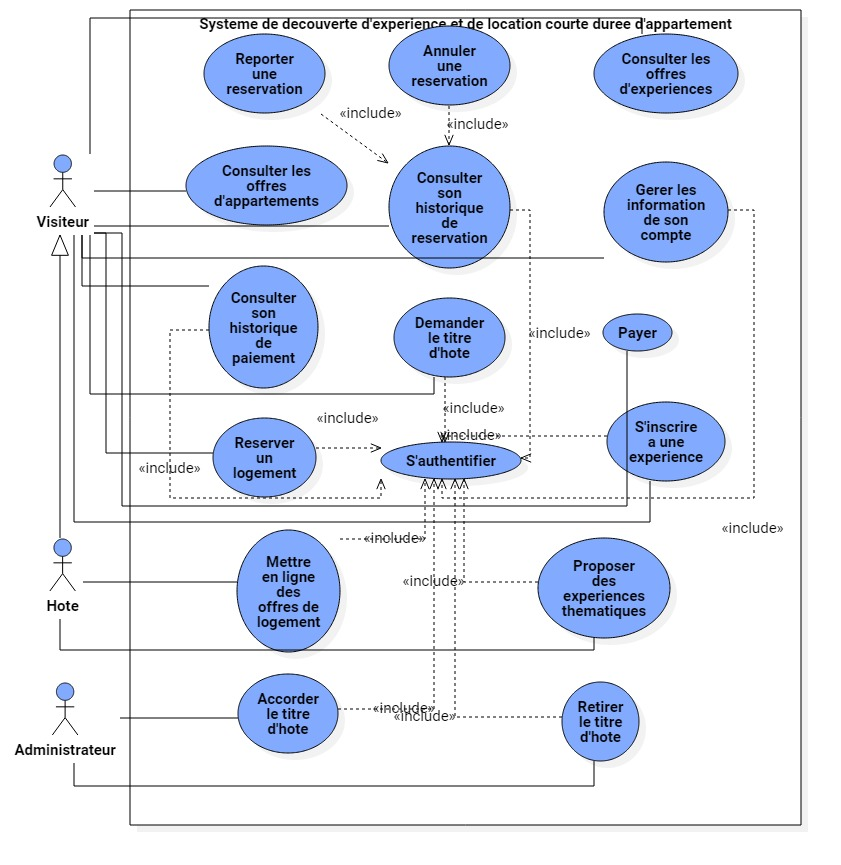
\includegraphics[width=18cm]{images/uml/UseCaseDiagram.jpg}
	\end{center}
	\caption{Diagramme de cas d'utilisation}
\end{figure}


\subsection{Analyse conceptuelle} 
\subsubsection{Diagramme des classes} 
Le diagramme des classes est considéré comme le plus important des diagrammes de la modélisation et de la structure interne du système. Il permet de fournir une représentation abstraite des objets du système qui vont interagir ensemble pour réaliser les cas d’utilisation.
\\$ $\\Notre étude a abouti au diagramme de classes suivant :
\begin{figure}[H]
	\begin{center}
		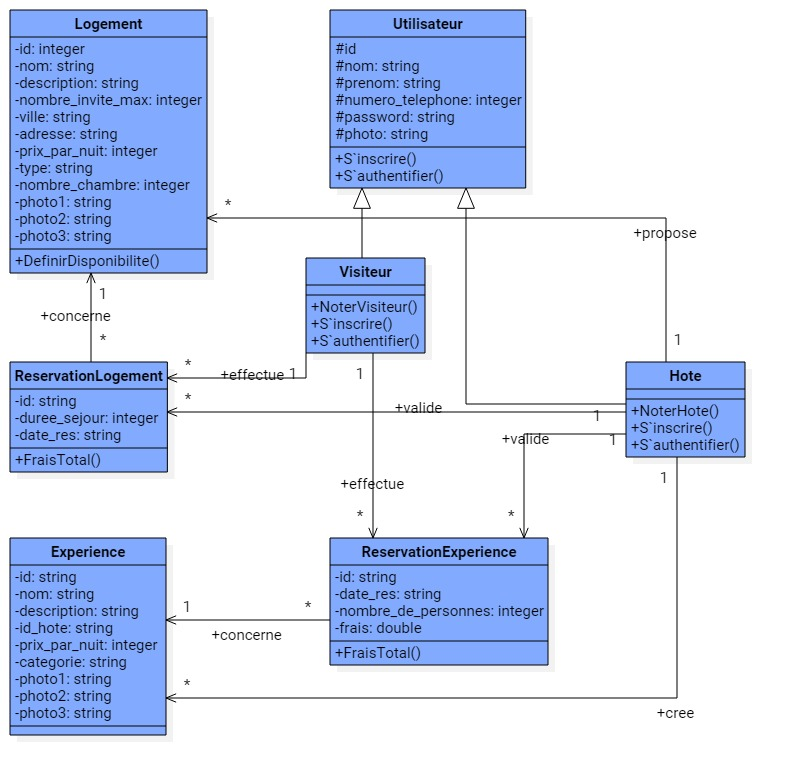
\includegraphics[width=18cm]{images/uml/ClassDiagram.jpg}
	\end{center}
	\caption{Diagramme des classes}
\end{figure}

\subsubsection{Diagramme de séquence} 
UML fournit les diagrammes d’interaction qui permettent de représenter la façon dont les objets réagissent via des messages. Il en existe deux (02) grands types : les diagrammes de séquence et les diagrammes de communication. Cependant, dans le cadre de notre domaine d’étude, nous allons présenter uniquement le diagramme de séquence.
\\Les diagrammes de séquences sont importants pour les raisons suivantes:
\begin{itemize}
\item[•] Ils permettent d'illustrer et vérifier le comportement d’un ensemble d’objet (système ou sous- système) ;
\item[•] Ils aident à la découverte des objets du système ;
\item[•] Ils aident à la découverte des méthodes des objets.
\end{itemize}

Nous allons présenter quelques diagrammes de séquences :
\begin{figure}[H]
	\begin{center}
		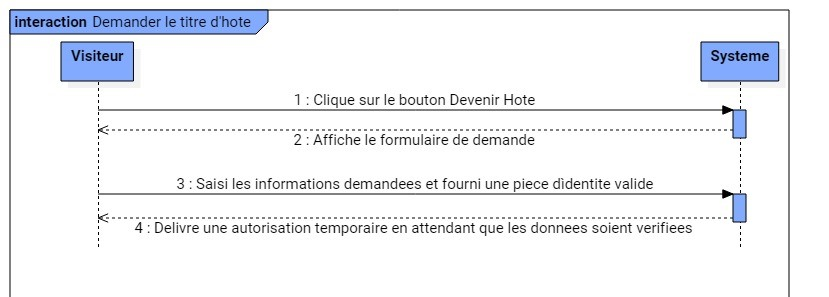
\includegraphics[width=18cm]{images/uml/SeqDemanderTitreHote.jpg}
	\end{center}
	\caption{Diagramme de séquence : Demander le titre d’hote}
\end{figure}
$ $
\begin{figure}[H]
	\begin{center}
		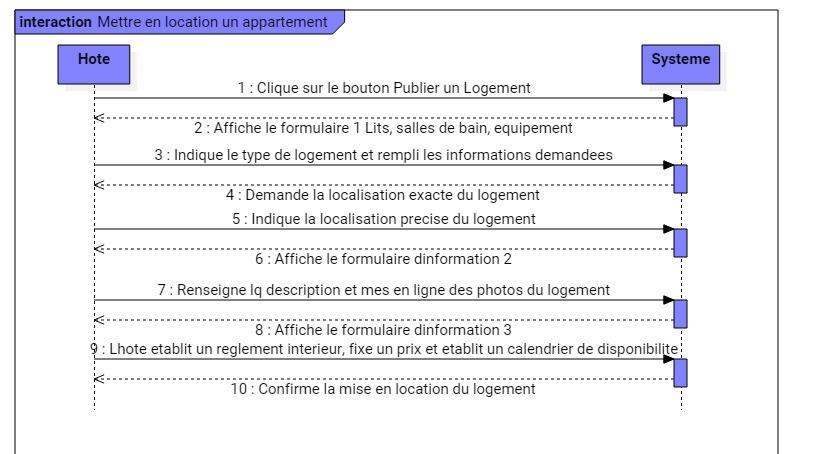
\includegraphics[width=18cm]{images/uml/SeqMettreLocationAppartement.jpg}
	\end{center}
	\caption{Diagramme de séquence : Mettre en location un appartement}
\end{figure}
$ $
\begin{figure}[H]
	\begin{center}
		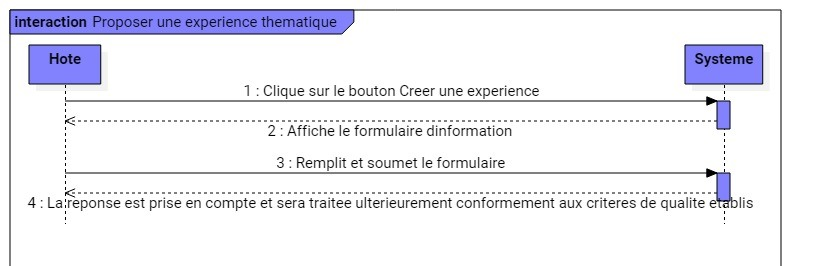
\includegraphics[width=18cm]{images/uml/SeqProposerExperienceThematique.jpg}
	\end{center}
	\caption{Diagramme de séquence : Proposer une expérience thématique}
\end{figure}
$ $
\begin{figure}[H]
	\begin{center}
		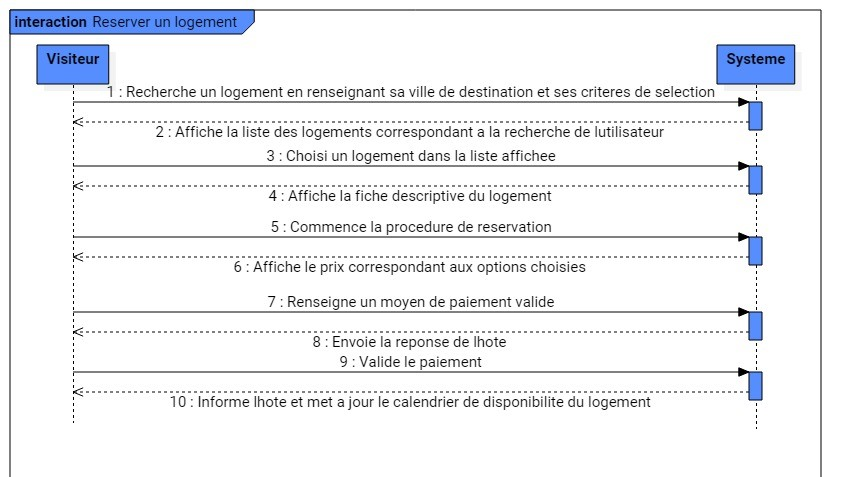
\includegraphics[width=18cm]{images/uml/SeqReserverLogement.jpg}
	\end{center}
	\caption{Diagramme de séquence : Réserver un logement}
\end{figure}
$ $
\begin{figure}[H]
	\begin{center}
		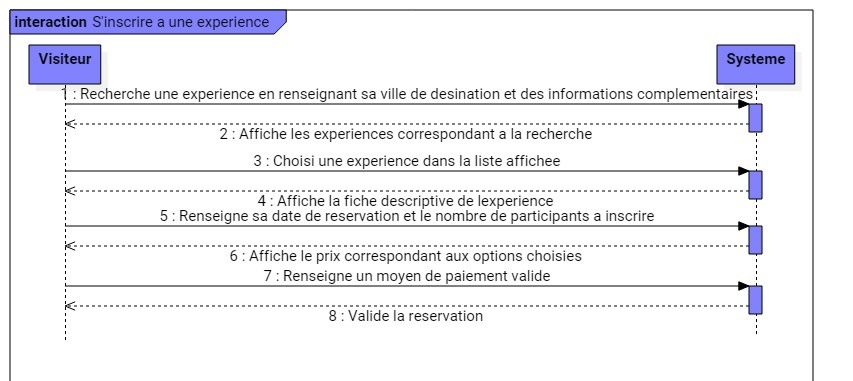
\includegraphics[width=18cm]{images/uml/SeqInscrireExperience.jpg}
	\end{center}
	\caption{Diagramme de séquence : S’inscrire à une expérience}
\end{figure}

\section{Choix des outils d'implémentation}
Cette partie présentera ensemble de technologies et outils que nous avons
mis en oeuvre dans l’implémentation de notre système.

\subsection{Architecture du système} 
Au vue du cahier des charges nous devrions produire au minimum deux applications qui partagent un ensemble d’informations mais pour différents publics. En effet nous devons récupérer un certains nombres d’informations du système de façon sécurisée et les distribuer aussi de façons contrôlée à la fois entre l’application mobile sur android et l’application web. De même ces deux applications devraient échanger entre elle un ensemble d’informations et de fonctionnalités propres au système à concevoir. 

Pour cela il faudrait déjà dans un premier temps qu’elles (les applications) partagent une base de données commune (centralisée), mais aussi un point d’entré commun pour accéder à cette base de données. Ce besoin nous amène donc à concevoir une interface de programmation au dessus du système d’information. Une architecture client serveur 3-tiers se décerne donc comme solution architecturale à notre cas. Cette dernière sépare l’application en 3 niveaux à savoir :

\paragraph{Niveau 1:} La couche présentation (ou affichage si l'on souhaite) associée au client qui de fait est dit "léger" dans la mesure où il n'assume aucune fonction de traitement.

\paragraph{Niveau 2:} La couche fonctionnelle liée au serveur, comprend le serveur d'applications ou middleware qui dans notre cas est un serveur Web interagissant avec la base de données et les clients.

\paragraph{Niveau 3:} La couche de données liée au serveur de base de données (SGBD).

Au coeur de cette architecture un composant dénommé API pour Application Programming Interface soit
Interface de programmation applicative devra fournir sous forme de services les
fonctionnalités qui ont trait à la logique du métier pour toutes nos applications clientes à conditions d'être autorisée. Ainsi toutes les fonctionnalités métier citées dans la partie application mobile et Application web doivent être développée au niveau de cette API. Les applications tierces à savoir l’application mobile et l’application web ne seront que de simple consommatrice de ces services.
De façon architecturale notre système ressemblerait ceci :
$ $
\begin{figure}[H]
	\begin{center}
		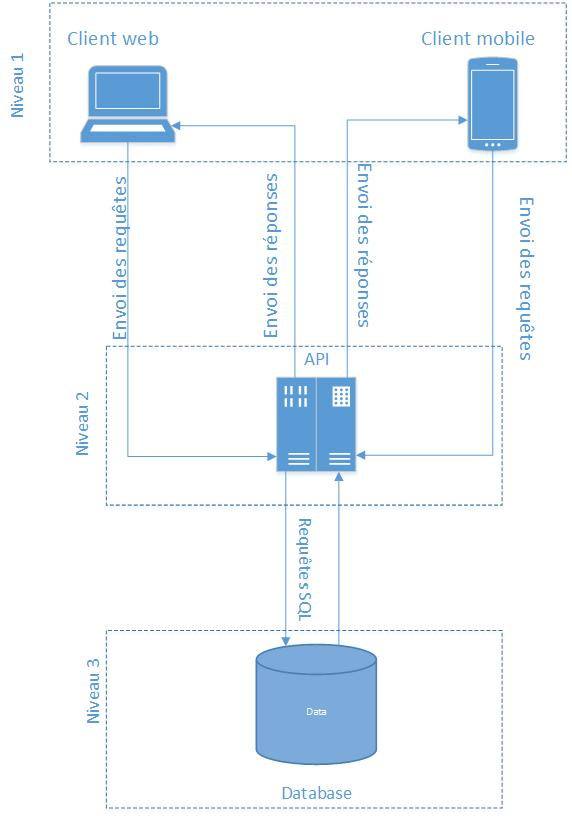
\includegraphics[width=14cm]{images/techno/3tiers.jpg}
	\end{center}
	\caption{Architecture du système}
\end{figure}
$ $
\subsection{Couche présentation} 
\subsubsection{Client Web}
\begin{figure}[H]
	\begin{center}
		
\includegraphics[width=14cm]{images/techno/mern.png}
	\end{center}
	\caption{MongoDB - ExpressJs - React - NodeJs}
\end{figure}
$ $\\Au niveau du client web nous utilisons la pile logicielle JavaScript moderne avec en son coeur le framework React en plus des langages classiques HTML et CSS respectivement dans leurs versions 5 et 3.
\begin{figure}[H]
	\begin{center}
		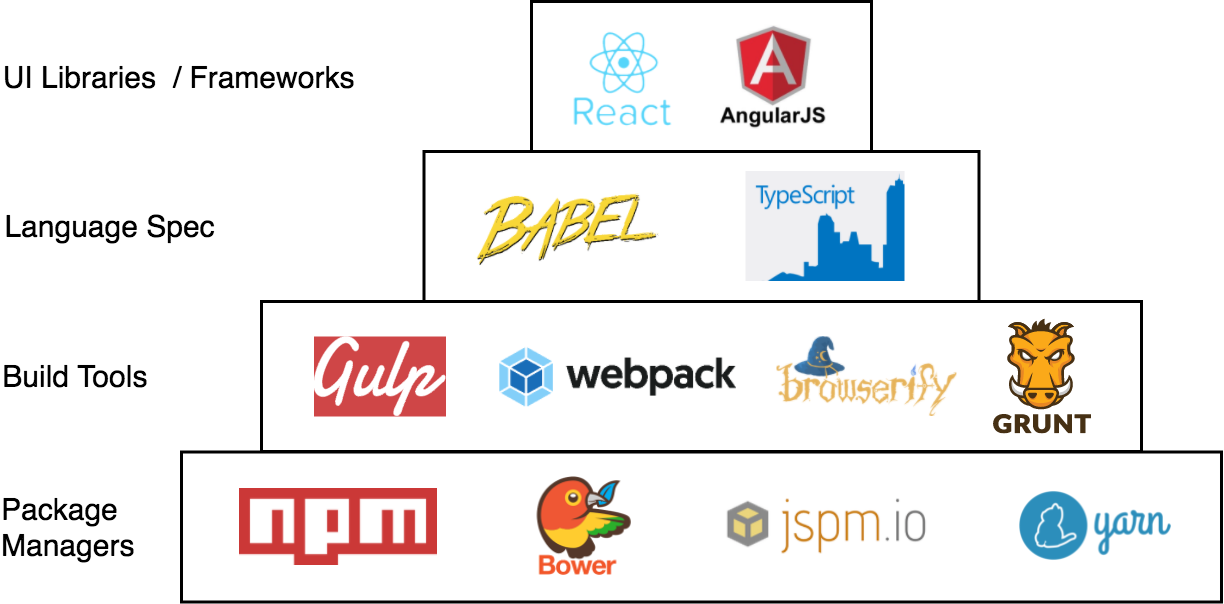
\includegraphics[width=10cm]{images/techno/jsarchi.png}
	\end{center}
	\caption{Moderne Stack Javascript}
\end{figure}

\paragraph{React.js} 
$ $\\Plus qu'une bibliothèque ou un framework, React est un paradigme de programmation d'interfaces utilisateurs, qui permet d'adresser de nombreuses plateformes, avec toujours du code React "standard".
\\Théoriquement, une application codée en React est capable de produire n'importe quel output, par exemple du HTML pour le web, du natif avec react-native, du WebGL, du terminal, de la musique...

\newpage
\subsubsection{Client Mobile}
$ $\\Le service a été pensé pour être accessible via un terminal mobile, indépendamment de la plateforme. Nous avons donc opté pour la réalisation d’une application mobile. Par conséquent il a fallu opérer un choix entre développement natif et hybride.
\\$ $\\Les applications natives, applications conçues spécifiquement pour un système d'exploitation, ont l'avantage d'offrir une expérience utilisateur et des performances optimisées pour leur plateforme spécifique. Cependant, la concentration sur une seule plateforme représente justement leur principal inconvénient. En effet, rendre la même application disponible sur une autre plateforme nécessite de la réécrire dans un langage spécifique à la plateforme choisie : Java ou Kotlin pour Android, Objective-C ou Swift pour iOS.
\\$ $\\Les applications hybrides quant à elles, se basent sur un même jeu de standards indépendamment de la plateforme choisie. Porter une application hybride vers plusieurs plateformes implique simplement de recompiler le même code source pour chacune d'elles. En contrepartie, elles offrent des performances moindres sur les terminaux les plus anciens et un accès limité à certaines fonctionnalités natives. Le souci de performance a longtemps limité leur pertinence. Cependant, de récentes avancées ont élargi leur champ de possibilités : Géo localisation, performances améliorées, accès à la caméra et au microphone, envoi de notifications, etc.
\\$ $\\Ces facteurs ont donc motivé le choix du développement hybride : Ionic, pour notre application client.
\subsubsection{Gestion de versions}
Nous terminerons cette partie par la présentation de Git un outil qui a été au cœur de notre travail de développement. Pour une bonne continuité dans l’implémentation et pour prévenir le risque que survienne un problème dans l’implémentation ou une perte des données du disque dur, nous avons besoin d’un gestionnaire de version. Notre choix s'est donc porté sur Git qui est un logiciel de gestion de version décentralisé. C'est un logiciel libre créé par Linus Torvalds, auteur du noyau Linux. En 2017, il s’agit du logiciel de gestion de versions le plus populaire qui est utilisé par plus de douze millions de développeurs (d’après Github). Comme Dépôt en ligne, nous avons utilisé la version communautaire de Gitlab avec des dépôts privés.

\subsection{Couche fonctionnelle} 
Elle permet d’assurer la transmission de la couche données vers la couche présentation, et inversement. Pour cela, il est fait recours à un middleware, sous la forme d’un web service. De nos jours, le standard REST est le plus répandu pour le développement des web services.
\\$ $\\REST (Representational State Transfer) ou RESTful est un style d’architecture permettant de construire des applications (Web, Intranet, Web Service). Il s’agit d’un ensemble de conventions et de bonnes pratiques à respecter et non d’une technologie à part entière. L’architecture REST utilise les spécifications originelles du protocole HTTP, plutôt que de réinventer une surcouche (comme le font SOAP ou XML-RPC par exemple). Une API compatible REST ou « RESTful » est une interface de programmation d'application qui fait appel à des requêtes HTTP. Dans cette architecture REST nous avons choisis le JSON comme format d'achat de données pour ça syntaxe souple qui favorise la rapidité des échanges.
\newpage
Nous avons choisi Node.js pour la réalisation de notre API REST. En effet, jusqu'ici, le JavaScript avait toujours été utilisé du côté du client, c'est-à-dire du côté du visiteur qui navigue sur notre site. Le navigateur web du visiteur (Firefox, Chrome, IE...) exécute le code JavaScript et effectue des actions sur la page web. Node.js nous permet d'utiliser le langage JavaScript sur le serveur.
\\$ $\\Au cœur de l’architecture node.js on retrouve des opérations IO non bloquantes, que ce soit à propos des interactions réseaux, ou de toutes les autres formes d’entrées/sorties, notamment le système de fichiers et les différentes bases de données aujourd’hui disponibles. C’est cet ensemble de bibliothèques IO non bloquantes, HTTP et autres protocoles de plus bas niveau (tcp, udp) que Node introduit au dessus du moteur JavaScript v8.
\\$ $\\Cet usage optimisé du matériel nous permet d’utiliser des serveurs plus léger sans avoir à sacrifier la performance aux yeux de l’utilisateur et ainsi traiter des milliers de requêtes simultanées, avec une empreinte mémoire faible.

\subsection{Couche données} 
Un Système de Gestion de Base de Données (SGBD) est un logiciel système destiné à stocker et à partager des informations dans une base de données, en garantissant la qualité, la pérennité et la confidentialité des informations, tout en cachant la complexité des opérations. Il permet d'inscrire, de retrouver, de modifier, de trier, de transformer ou d'imprimer les informations de la base de données.

\paragraph{MySQL} 
$ $\\MySQL est un serveur de bases de données relationnelles SQL développé dans un souci de performances élevées en lecture, ce qui signifie qu'il est davantage orienté vers le service de données déjà en place que vers celui de mises à jour fréquentes et fortement sécurisées. Il est multi-thread et multi-utilisateur. C'est un logiciel libre, open source, développé sous double licence selon qu'il est distribué avec un produit libre ou avec un produit propriétaire.

\paragraph{PostgreSQL}
 $ $\\PostgreSQL est un système de gestion de bases de données relationnel robuste et puissant, aux fonctionnalités riches et avancées, capable de manipuler en toute fiabilité de gros volumes de données, même dans des situations critiques. Il est de type SQL et extrêmement respectueux des standards, se conformant au plus près à la norme ANSI-SQL 2008.

\paragraph{MongoDB}
$ $\\MongoDB (de l'anglais humongous qui peut être traduit par « énorme ») est un système de gestion de base de données orientée documents, répartissable sur un nombre quelconque d'ordinateurs et ne nécessitant pas de schéma prédéfini des données. MongoDB est développé depuis 2007 par MongoDB et fait partie de la mouvance NoSQL (Not Only SQL). MongoDB permet de manipuler des objets structurés au format BSON (JSON binaire), sans schéma prédéterminé. En d'autres termes, des clés peuvent être ajoutées à tout moment « à la volée », sans reconfiguration de la base.

\paragraph{Choix}:
$ $\\Notre choix s’est porté sur MongoDB. La raison principale de notre orientation est que c’est le SGBD que nous avons eu a utiliser durant notre stage aussi bien en développement qu’en production\footnote{www.mongomanager.space}. De plus, pour stocker les données de traitement de notre système nous avons utilisé une base de données NoSQL “Not only SQL” pour sa scalabilité horizontale\footnote{La scalabilité verticale implique d’augmenter les ressources de calcul de chaque serveur composant l’infrastructure tandis que la scalabilité horizontale, consiste à multiplier les nœuds de calcul au niveau le plus bas de l’infrastructure et à configurer les logiciels de middleware pour qu’ils s’exécutent sur de multiples hôtes redondants de manière à assurer une répartition optimale de la charge (load-balancing)} et sa capacité à permettre la gestion de volumes de données importants. NoSQL permet également des traitements plus rapides pour certains types d'applications.


\section{Sécurité de l’application}
Le système que nous avons développé traite des informations sensibles : les données personnelles et banquaires des utilisateurs. A partir du moment ou nous faisons transiter ces informations
entre différents réseaux et interconnectant différentes applications nous devrions
prendre des mesures sécuritaire pour réduire autant que possible les failles de
sécurité.
$ $\\Nous classons ci-dessous les mesures que nous avons adoptées en fonctions
des principes de sécurité informatique :
\subsection{La confidentialité}
La confidentialité est le fait de s’assurer qu’une information est accessible
uniquement par les entités qui ont le droit d’accéder à celle-ci.
Le système que nous avons développé intègre cet aspect de la sécurité à deux
niveaux :
\begin{itemize}
	\item[\textbullet] Dans un premier temps nous avons installer un certificat ssl de 2048 bits
	qui nous permet de sécuriser toutes les communications utilisant le
	protocole tcp/ip.
	\item[\textbullet] Dans un second temps un système de gestion de rôle et de droit intégré
	nous permet de respecter la confidentialité des données dans chaque sous
	système. En effet chaque utilisateur appartient à un groupe
	d’utilisateurs donné et pour chaque groupe seulement un ensemble
	d’actions bien définies sont possibles.
\end{itemize}
\subsection{L’Intégrité}
L’intégrité s’assure que la donnée reste toujours intègre c’est-à-dire
qu’elle n’a pas été modifiée par un tiers non autorisé. Cet principe de sécurité
est pris en compte par la mise en place d’un certificat ssl sur le serveur
d’applications.
\subsection{La disponibilité}
La disponibilité est le fait de s’assurer que l’information soit toujours
disponible peu importe le moment choisit.
$ $\\Elle a été assurée en partie par l'infrastructure mise en place comme des
serveur de redondance mais aussi par la virtualisation des ressources et des
applications qui ont été déployées. Aussi une gestion de la montée en charge a
été prévue mais n’a pas été implémenté.
\subsection{L’Authenticité}
Au sein d’un système d’information, il est important de vérifier
l’authenticité de chaque ressource. Cela est possible grâce au mécanisme
d’authentification, qui permet de prouver l’identité d’une personne via le
processus d’identification.
$ $\\A notre niveau nous avons mis cela en place par une forte authentification
à deux niveaux. Dans un premier temps avant de faire appel à une quelconque
URI il faudrait être authentifié avec un couple d’identifiant comme service tiers
de confiance. Donc nos applications clientes s’authentifient avant de demander
un quelconque service au Backend. Après être autorisé les applications clientes
ont le devoir d’authentifier leurs utilisateurs avant de pouvoir faire une
opération (lecture ou écriture) mettant en relation un utilisateur du système.
$ $\\Bien qu’ayant installé un certificat sur le serveur nous évitons de faire
circuler les paramètres de connexion de l'utilisateur. En lieu et place nous avons
utilisé un jeton qui est une longue chaîne de caractères générée et encryptée
automatiquement lors de l’authentification de l’utilisateur. C’est désormais cette
clé renouvelable et ayant une durée de vie limitée qui est désormais envoyé
conjointement avec les requêtes pour authentifier l’utilisateur. Toute requêtes ne
contenant pas de jeton ou contenant des jetons invalide sont automatiquement
rejetées.
\subsection{Non-répudiation}
La non-répudiation se base sur un principe simple : une entité ne peut nier
son implication dans une action à laquelle il a participé.
$ $\\Dans notre cas la non-répudiation peut être atteinte seulement en utilisant la
technologie du certificat numérique avec un chiffrement asymétrique.
\subsection{Imputabilité}
Il s’agit des techniques mises en oeuvres pour assurer la traçabilité des actions
d’un individu sur un système. Nous avons mis en place cette traçabilité en
journalisation toutes les actions menées sur les objets du système.